\documentclass[../main.tex]{subfiles}
\graphicspath{{\subfix{../figures/}}}

\begin{document}

\chapter{Preliminaries}

\section{Gene Expression Regulation}

Across all cells genetic information flows from DNA to RNA to proteins, the central dogma of molecular biology \parencite{Crick1970}.
Transcription from DNA to RNA and translation from RNA to protein are regulated by numerous mechanisms simultaneously to enable cells to respond to their environment.
This chapter is a brief overview of the transcription and post-transcriptional regulatory mechanisms that contribute to the differential expression of mRNA transcripts with emphasis on the mechanisms present in \textit{Saccharomyces cerevisiae}, Figure \ref{fig:mrna-regulation}. 

\begin{figure}[h]

{\centering 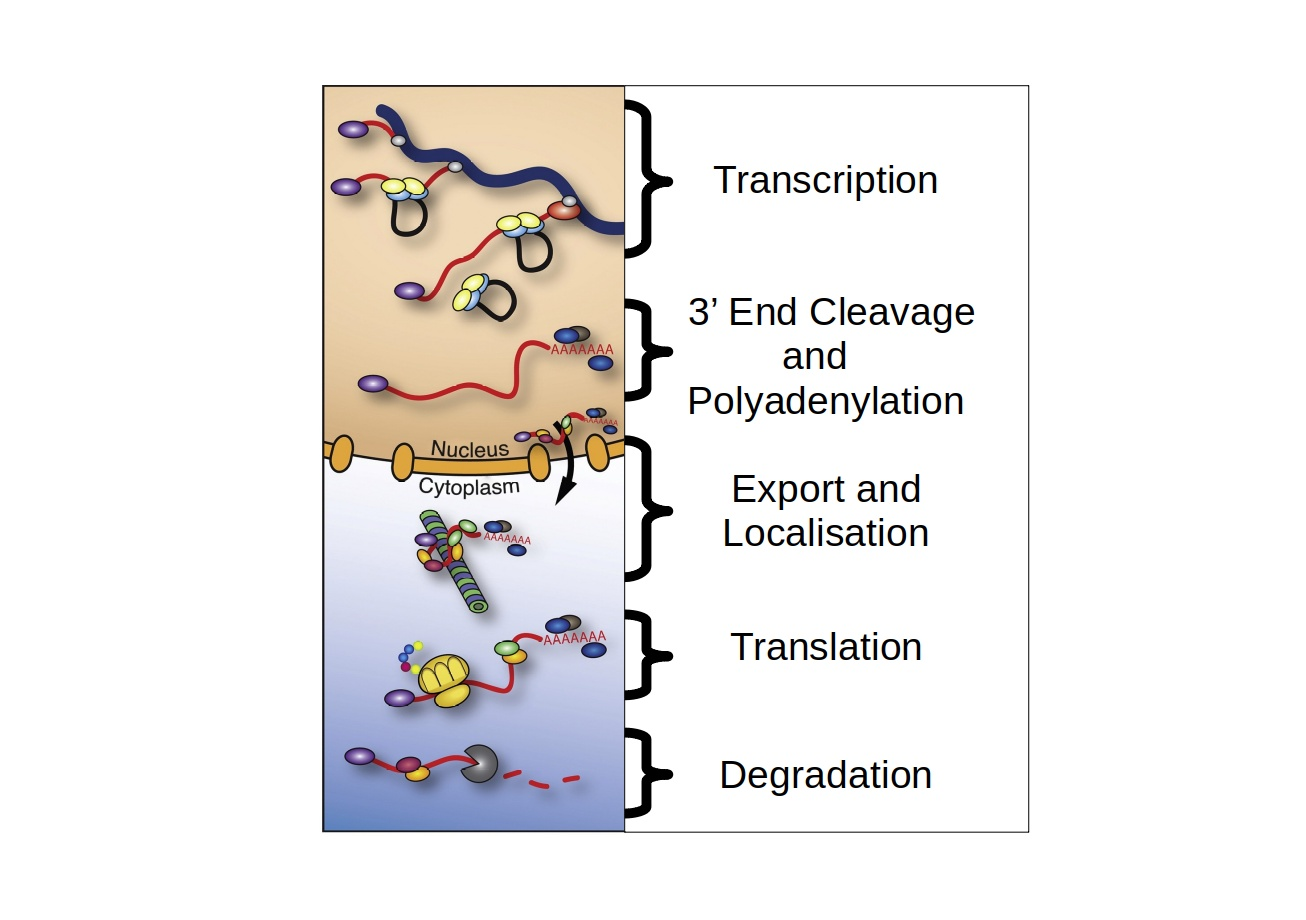
\includegraphics[width=\linewidth]{figures/post-transcriptional-regulation} 

}

\caption[Overview of key mRNA regulatory processes.]{\textbf{Overview of key mRNA regulatory processes.} Several mechanisms act simultaneously to enable cells to respond to their environment through the regulation of mRNA transcripts. Figure adapted from \cite{Corbett2018}}\label{fig:mrna-regulation}
\end{figure}


\subsection{Transcriptional regulation}

The creation of an mRNA transcript from a DNA template requires the completion of three key transcriptional steps: initiation, elongation and termination.
Initiation of mRNA transcription consists of the RNA polymerase II binding to the DNA template upstream of the sequence encoding a protein.
The region where the RNA polymerase II initiates transcription is called the promoter.
In eukaryotes, DNA is wound around nucleosomes and densely packaged in several orders of chromatin structure.
Therefore, the initiation of transcription requires a variety of transcription factors to aid in the unwinding of the chromatin, scanning of regions for promoters, and the binding of RNA polymerase II.
Promoters consist of regulatory sequences that encourage the binding of transcription factors and can be further affected by distal regulatory regions such as enhancers \parencite{Cramer2019}. 

Once transcription is initiated the polymerase begins the sporadic process of elongation from the transcript start site.
The polymerase first transcribes the 5' untranslated region (5'UTR) of an mRNA transcript, then the coding sequence for the corresponding protein, and finally the 3' untranslated region (3'UTR).
For genes that contain introns, the polymerase will also transcribe the intron sequences which can occur across the nascent transcript but are removed from the mature mRNA transcript.  
The process of elongation is highly stochastic with polymerases regularly pausing and even stalling with several accessory proteins required to maintain the process.
Early on in the elongation stage, the 5' end of the pre-mRNA is modified by several enzymes to form a 5'-methyl cap which inhibits degradation and aids translation.
Finally, the termination of transcription remains a relatively unclear process as a distinct termination sequence has not been found.
Instead, the polymerase continues to transcribe the sequence downstream of the 5'UTR.
This downstream terminator region does contain sequences to recruit cleavage and polyadenylation factors.
The still elongating RNA transcript is cleaved at the end of the 5'UTR as dictated by these sequences.
The freely floating pre-mRNA transcript is then bound by a poly(A) polymerase that adds a tail of hundreds of adenine bases to the end of the transcript.
The remaining string of RNA bound to the polymerase and DNA template is degraded by a 5' to 3' exonuclease, which is thought to dislodge the polymerase and terminate transcription \parencite{Alberts2017,Cramer2019}.
The terminator can contain multiple cleavage sites leading to transcript variants, called isoforms, with different poly(A) positions.
Transcript isoforms can also be created as the promoter can contain different transcription start sites leading to transcript isoforms with different coding sequences and 5'UTRs \parencite{Klerk2015}.

\subsection{Post-transcriptional regulation}

A variety of regulatory mechanisms act in between the transcription of a nascent mRNA transcript and its translation into a sequence of amino acids.
Key tasks include: removing introns, conducting quality control and transporting transcripts around the cell.
Introns are regions that are transcribed but are not in the final mature mRNA transcript.
Concurrently with or immediately after transcription a group of co-functional RNA and proteins called the spliceosome remove intron segments within nascent RNA transcripts.
The regions that forms the mature mRNA transcript are called exons and a single transcript may consist of 10's of exons spliced together.
Alternative splicing of introns and exons can theoretically produce thousands of different versions of a protein in some Drosophila genes \parencite{Wilkinson2020}.

Selective degradation of low quality mRNA or transcripts that that are no longer needed is a crucial post-transcriptional regulation mechanism.
The importance of degradation in gene regulation is reflected in the number of redundant processes to degrade transcripts, but the majority of degradation is facilitated by the deadenylation-dependent mRNA decay pathway.
This pathway starts by flagging transcripts for degradation by shortening  the poly(A) tail.
Then, either the 5'methyl cap is removed to enable 5'->3' degradation by the XRN1 exoribonuclease or 3'->5' degradation is initiated by the exosome attaching to the exposed 3' end. 
A variety of surveillance methods can trigger transcript degradation, including: non-sense mediated decay which checks for premature stop codons, non-stop mediated decay which checks for missing stop codons, and no-go mediated decay which checks for stalled ribosomes on mRNA.
In response to stress or other causes of high load on the degradation machinery, P-bodies can form in the cytoplasm that are believed to facilitate degradation as they often contain deadenylation, decapping and degradation factors \parencite{Garneau2007}.

Spatial regulation enables centrally transcribed mRNA transcripts to be regulated differently depending on the target location of their encoded protein.
In budding yeast, the Ash1 protein represses mating-type switching, but only in daughter
cells \parencite{Sil1996}.
The localisation of the ASH1 transcript at the bud tip and subsequent localised translation ensures the Ash1 protein is not present in the parent cell despite being transcribed in its nucleus \parencite{Niednery2014}. 
It is thought that co-transcriptional recruitment of She2 protein to the Ash1 transcript in the nucleus of the parent cell enables the later recruitment of cytoplasmic factors Khd1/Hek2 and Puf6, factors known for translational repression. 
Furthermore, successful transport of ASH1 to the bud tip by She2-She3-Myo4 complexes depends on translational repression by Khd1 and Puf6. 
Later, phosphorylation of Khd1 and Puf6 by bud-membrane-localised kinases leads to localised translational activation of the ASH1 mRNA \parencite{Paquin2007, Deng2008}.

Another example where the effect of a CRE on a transcript depends on co-localisation with a regulatory kinase comes from the fungal RNA-binding protein Ssd1. 
Yeast cell wall proteins such as Sun4 and Tos6 are translationally repressed by Ssd1 \parencite{Jansen2009}.
It is thought that these transcripts are translationally activated at bud sites after the phosphorylation of Ssd1 by a localised kinase, Cbk1 \parencite{Jansen2009, Kurischko2011}. 
There is no evidence that Ssd1 directly acts to transport RNA, so this localised activation presumably depends on localisation the recruitment of other RNA-binding proteins to those transcripts \parencite{Hogan2008, Bayne2021}, that then recruit transport machinery.

Post-transcription regulation is also known to facilitate temporal regulation in cells.  
Temporal regulation is common in developmental processes where the order of production of specific proteins is highly regulated. 
For example, in C. elegans lin-4 is a non-coding RNA gene crucial for regulating cell fates during the early stages of larval development \parencite{Wightman1993}. 
Lin-4 is a small RNA that binds to its target mRNA lin-14 and inhibits the translation of lin-14 \parencite{Lee1993}.
Since lin-4 is only expressed at the end of the first larval development stage, lin-14 is only translationally inhibited at the end of stage 1, initiating the start of stage 2 \parencite{Olsen1999}. 
Similarly, to establish meiotic chromosome segregation in budding yeast, mRNA encoding cyclin CLB3 is transcribed in stage I of meiosis, but is translationally repressed until stage II of meiosis. 
CLB3 is translationally repressed by the RNA-binding protein Rim4. 
During the transition to meiosis II, Rim4 is phosphorylated which inhibits binding to CLB3 and enables CLB3 to be translated \parencite{Berchowitz2013}. 
Therefore, post-transcription control of CLB3 by Rim4 and of lin-4 by lin-14 depends on the timing of promoter-specified transcriptional control.

\newpage


\section{Experiments Quantifying RNA Abundance}

\subsection{qPCR}

Quantitative polymerase chain reaction (qPCR) is the basis of countless assays that can quantify various populations of DNA and RNA.
Polymerase chain reaction (PCR) is regarded as one of the most significant methods in molecular biology as it enables the production of copies of regions of DNA. 
The log-linear growth of copies from PCR duplication led researchers to explore its use as an accurate method to quantify abundance \parencite{Saiki1988}.
After its invention in the 1980's the quantification of the rate of amplification in real time quickly followed \parencite{Holland1991}, but it was not until the 2000's that biochemistry and technology matured into a reliable quantitative PCR (qPCR) method \parencite{Walker2002}.
qPCR is a relatively low-throughput quantification method when compared to the other methods described here.
However, developments in microfluidics and multiplexing target probes are overcoming the bottlenecks in conducting high-throughput qPCR \parencite{Dreier2022}.

The basic principle of PCR consists of the duplication of a region of DNA that is specified by two short nucleotide sequences, called primers, that are designed to be complementary to the start and the end of the region of interest. 
A highly thermotolerant polymerase, adapted from the bacteria \textit{Thermus aquaticus}, is then able to complete the duplication of the region by elongation of the sequence between the two primers \parencite{Saiki1988}.
The duplication cycle is repeated several times leading to an exponential growth in the number of copies of the original region.
The PCR polymerase must be thermotolerant as the duplication cycle is rapidly repeated by raising the temperature to melt the newly created complementary strand away from the original strand before dropping the temperature back down to enable the next round of elongation. 
Quantifying the rate of amplification, is done by introducing dyes that only fluoresce when a region has been successfully duplicated. 
The fluorescence of the sample is measured as the PCR cycle is repeated to determine the exponential growth in duplicates.
Quantitative PCR (qPCR) uses the amplification curve to infer the number of transcripts of the target sequence in the original sample \parencite{Holland1991}.

\subsubsection{qPCR methods: RNA vs DNA}

qPCR is highly optimised for amplifying DNA fragments using engineered derivatives of the \textit{Thermus aquaticus} polymerase \parencite{Witte2018}. 
Therefore, to quantify RNA fragments an additional step is required to create complementary DNA (cDNA) from RNA using a reverse transcriptase. 
Unfortunately, this step can be a significant source of variation and has been determined to be the source of most variation between RNA samples. 
The variation in cDNA yield between replicates can be influenced by the choice of reverse transcriptase priming method, the original RNA target concentration and the total RNA concentration in the sample. 
In order for a RT-qPCR experiment to be reproducible the reverse transcriptase step must be optimised and clearly described \parencite{Stahlberg2004}. 

\subsubsection{qPCR methods: Intercalating dyes vs probe-specific dyes}

\begin{figure}[h]

{\centering 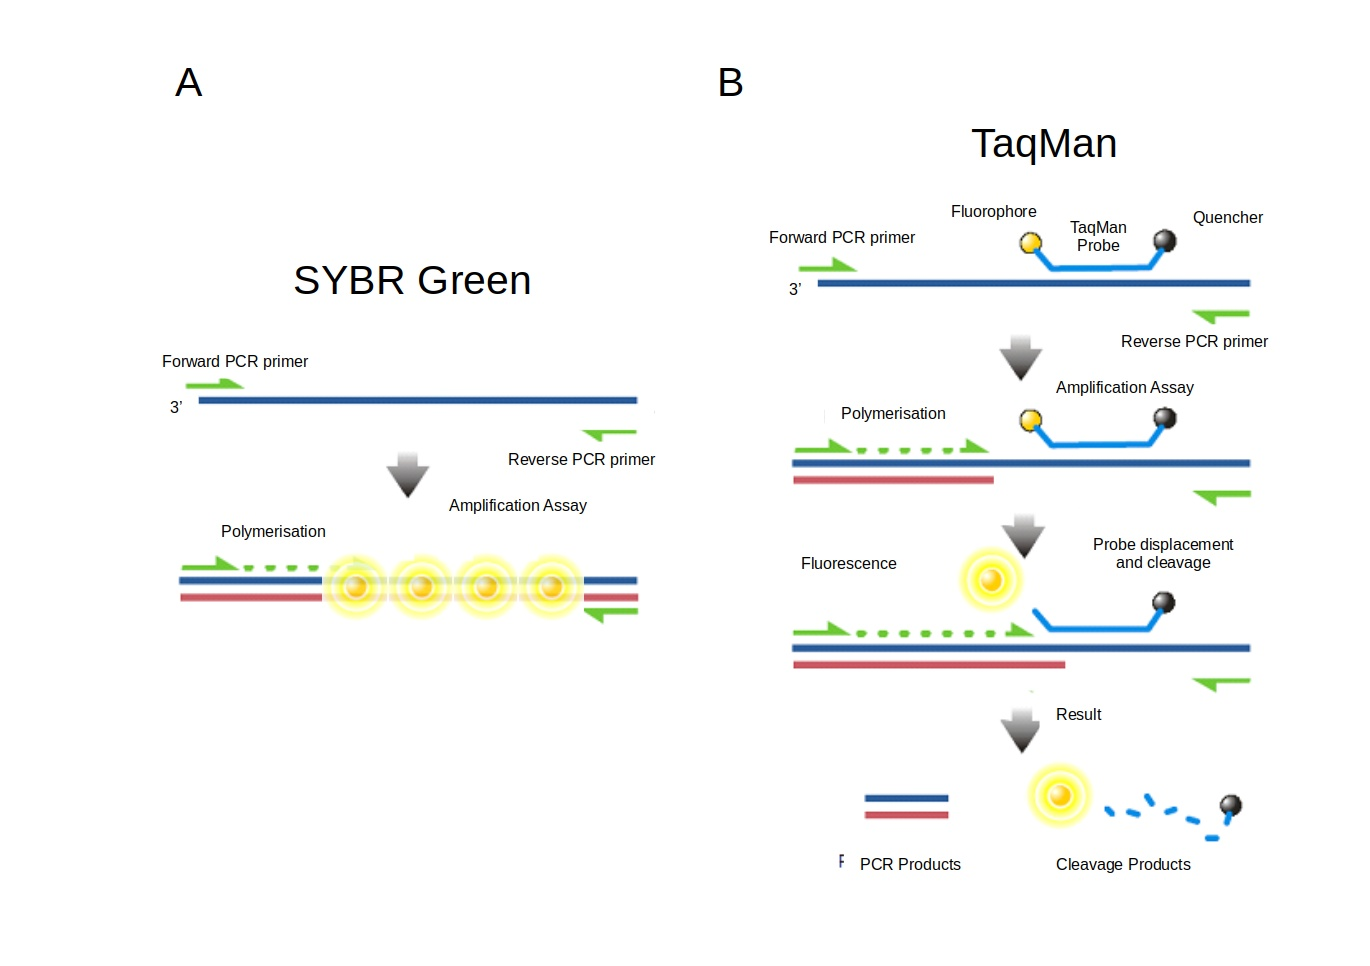
\includegraphics[width=\linewidth]{figures/taqmanvssybrgreen} 

}

\caption[Key steps in a qPCR assay.]{\textbf{Comparison of the key steps in a qPCR assay using two different fluorescent probes.} (\textbf{A}) Intercalating dyes, such as SYBR Green fluorescent probes, bind to any double stranded DNA. (\textbf{B}) Probe-specific dyes, such as TaqMan fluorescent probes, bind to specific sequences and only fluoresce once detached from their paired quencher during elongation. Figure adapted from Wikimedia Taqman diagram.}\label{fig:qpcr-fluo-tech}
\end{figure}

% https://commons.wikimedia.org/w/index.php?curid=42613619

There are two common types of fluorescent dye used to measure duplicated fragments: probe-specific dyes vs intercalating dyes.
Intercalating dyes fluoresce when they bind to any double stranded DNA species in a sample \parencite{Ihmels2005}, Figure \ref{fig:qpcr-fluo-tech}A.
This leads to it being a cheap and relatively easy to use system, but it is highly susceptible to contamination and it is unable to distinguish between samples from different targets. 
Probe-specific dyes bind the fluorescent dye to a oligonucleotide probe that is designed to attach to the region of interest somewhere in between the two primers. 
The oligonucleotide probe has the fluorescent dye on one end and a quencher on the other.
The quencher stops any excitation emissions from the dye through fluorescence resonance energy transfer \parencite{Juskowiak2010}. 
However, during elongation, when the polymerase reaches the oligonucleotide probe it is hydrolysed separating the dye from the quencher.
Emissions from the fluorescent dye can then be measured and the creation of a new duplicate is detected, \ref{fig:qpcr-fluo-tech}B. 
The introduction of a custom oligonucleotide probe increases the specificity of probe-specific dye methods and reduces the effects of contamination. 
Also, the abundance of multiple targets can be measured in the same sample by carefully designing different oligonucleotide probes with different fluorescent dyes.
Unfortunately, the design and creation of custom probes causes probe-specific dye methods to be more expensive and technical \parencite{Adams2020}. 
The accuracy of the cheaper intercalating dyes methods and the probe-specific dye methods is comparable, if correctly conducted \parencite{Tajadini2014}.
Although, the limit of detection (LOD) of low copy targets depends on protocol optimisation. 

\subsubsection{Quantifying abundance: Curve fitting vs cycle threshold}

The exponential limit of the number of duplicates per cycle enables methods that compare abundance across samples. 
Assuming all samples reach the exponential growth stage at the same time then the difference in fluorescence at any cycle of the PCR assay is dependent only on the original copy number. 
However, even if the duplication is perfectly efficient, the amplification curve of duplicates per cycle is not a perfect exponential as there is a limited window through which the number of duplicates will grow exponentially.
The window is defined by limitations in detecting fluorescence at low abundance and the exhaustion of resources at high abundance.
The original copy number can be inferred from the fluorescence if you set a particular fluorescence threshold during the exponential phase and compare the number of cycles needed for a sample to reach it.
Unfortunately, this method assumes both that each sample reaches the exponential phase at the same time and that each cycle doubles the number of duplicates perfectly for each sample \parencite{VanGuilder2008}. 
An alternative method fits an sigmodal curve to the amplification curve and uses this model to deduce the cycles required to reach a the threshold.
The additional fitting can account for difference in the times to reach the exponential growth phase between samples and can directly account for deviations in perfect duplication \parencite{Swillens2008}. 

\subsubsection{Quantifying Abundance: Relative vs absolute}

Multiple methods exist for converting cycle threshold measurements, Cq, into quantitative values for sample abundance whilst accounting for experimental and technical noise.
First, qPCR experiments can be designed to measure the relative change in abundance across samples.
Relative abundance measurements depend on the determination of genes that have constant expression across all samples/conditions.
Any change in the gene(s) of interest across samples can then be detected by comparing $\Delta$Cq or the expressions relative to the set of constantly expressed genes.
Normalising the fluorescence to genes with constant expression minimises batch effects introduced by sample preparation, reverse transcription and reactants.
Alternatively, the absolute number of copies of a target in a sample can be estimated.
Absolute quantification of a target requires a preliminary experiment where known initial quantities of the gene of interest are measured with qPCR.
Several amplification curves for the gene of interest, with gradually increasing copies of the gene of interest, are measured to create a collection of standard curves.
Next, the sample from the primary experiment is measured with qPCR and its amplification curve is compared to the standard curves.
The absolute copy number of the gene of interest in the experimental sample can then be interpolated \parencite{Wong2005, VanGuilder2008}.

\subsection{Microarrays}

Microarrays facilitated the creation of the some of the first high-dimensional data sets in transcriptomics.
In the 1980's an assay was published to simultaneously determine multiple specific cell surface antigens through the use of a matrix of antibodies fixed to a glass slide \parencite{TseWen1983}.
The opportunity to quantify multiple characteristics of a sample using the same chip led other labs to explore attaching oligonucleotides to a slide, inventing microarrays \parencite{Schena1995}.
The technology enabled the abundance of thousands of genes to be measured simultaneously unlocking genome wide studies of gene expression regulation across conditions \parencite{Gasch2000}. 
The assay also benefited from the high quality sequencing of the genomes of multiple species as oligonucleotide probes could be designed to investigate any regions of interest \parencite{Lander2001}.

Microarrays consist of a glass or silicon substrate with spots of DNA printed on in a regular grid. 
Each DNA spot is a complement to a different target which fluoresces when bound with the target. 
In assays to determine differential expression, two colour microarrays are used where each spot contains two fluorescent probes; one to detect the target abundance in the sample of interest and one to detect target abundance in a control or another sample of interest.
A camera detects the level of fluorescence across each spot after excitation by a laser which is used to determine the abundance of that target.  
The two colour microarray assay measures the fluorescence of the two fluorophores and uses the ratio to determine changes in expression.
As the DNA probes have to be designed and printed onto the glass plate their complementary targets have to be decided before conducting the experiment which reduces the opportunity to discover novel regulatory elements \parencite{Schena1995}.
Microarrays facilitated the development of high-throughput transcriptomic experiments as RNA transcript abundance can also be investigated by introducing a reverse transcriptase step to create cDNA fragments. 

\subsection{RNA-Seq}

The success of the microarray was limited by the requirement of specifying the target probes prior to the experiment.
However, its densely packed array of oligonucleotides fixed to a solid surface inspired a new sequencing method.
For 30 years the primary method for sequencing unknown DNA fragments was Sanger sequencing with its successful application in decoding the human genome \parencite{Lander2001}. 
The method consists of introducing a di-deoxynucleotide triphosphate (ddNTP) version of one of the four nucleic acids which induces premature termination of elongation when the polymerase incorporates it into a DNA chain.
Due to the stochasicity of elongation the introduction of ddNTP occurs at different stages of duplication leading to the creation of a population of different lengths of copies of a target.
Separating the population by weight using electrophoresis creates bands where the chosen nucleic acid has been replaced by a ddNTP version.
Repeating the process by replacing each nucleic acid in turn enabled a target sequence to be decoded \parencite{Sanger1977}.
Similar to qPCR, Sanger sequencing can also be extended to RNA sequencing by introducing a reverse transcriptase step to make cDNA.
The accuracy of the Sanger method means it is remains in use today, but the cost and difficulty of scaling up the method has limited it use.

\begin{figure}[h]

{\centering 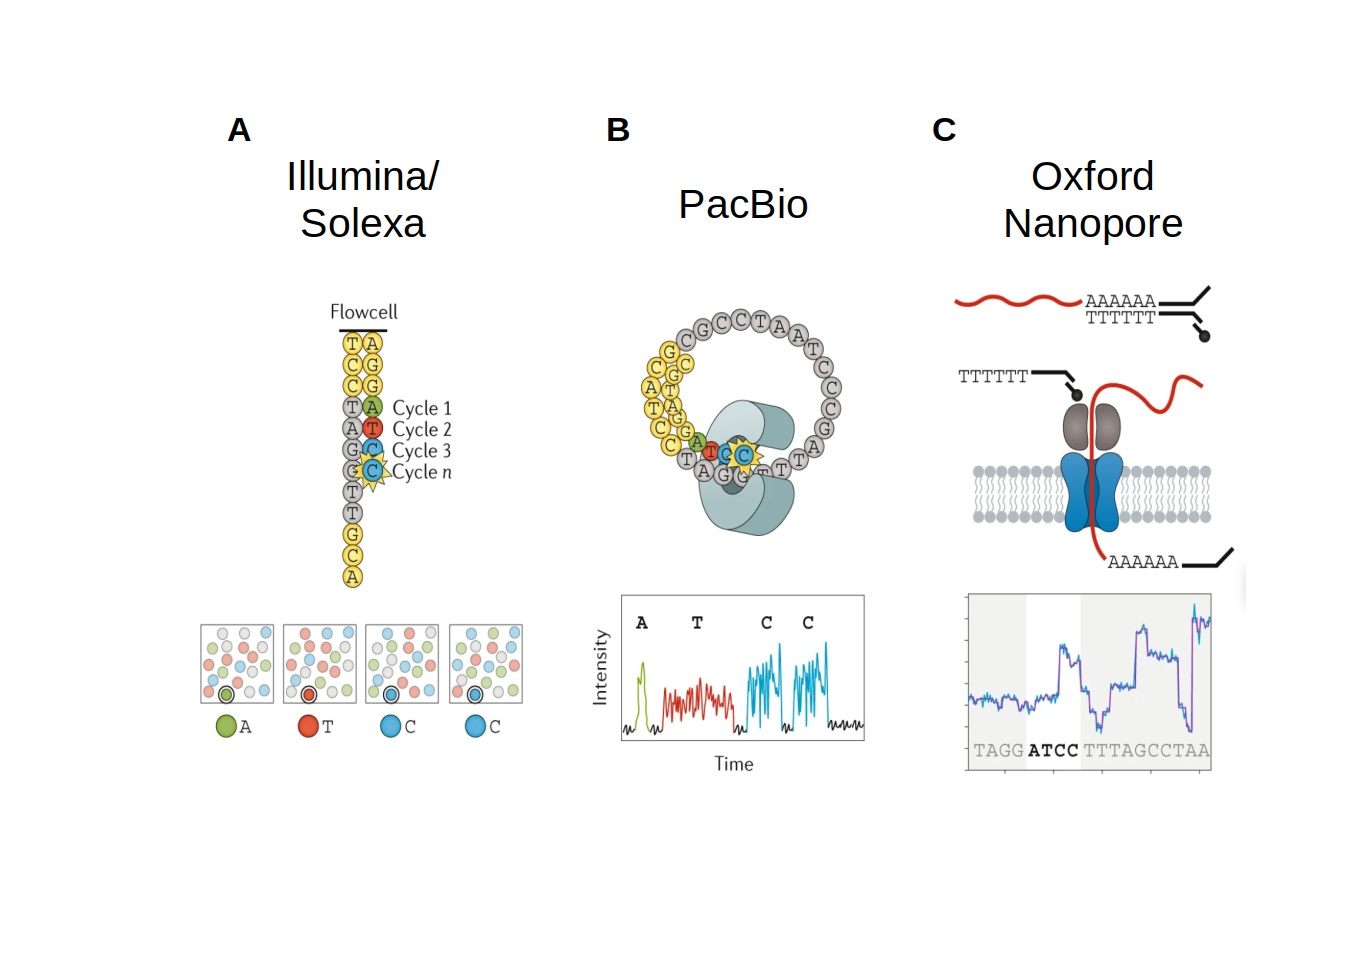
\includegraphics[width=\linewidth]{comparisonofsequencers} 

}

\caption[Comparison of RNA-Seq technologies.]{\textbf{Comparison of RNA-Seq technologies.} (\textbf{A}) Illumina sequencers attach short fragments to a solid surface called a flowcell. Fluorescent nucleotides create a clear fluorescent spot that identifies the last nucleotide to be attached. (\textbf{B}) PacBio sequencers enable long reads by opening up double stranded DNA into a circle. A polymerase can loop round the circle attaching fluorescent nucleotides that identify the next nucleotide in the sequence. (\textbf{C}) Oxford Nanopore sequencers force nucleotide fragments through protein pores in a membrane. The transmembrane proteins change the current passing through them in response to the nucleotide sequence. The changing in the current can be used to determine the nucleotide sequence. Figure adapted from \cite{Stark2019}}\label{fig:rna-seq-tech}
\end{figure}

\subsubsection{Shotgun sequencing}

In the early 2000's, several companies competed to overcome the microarray's deficiency in requiring DNA targets to be defined before the experiment \parencite{Rusk2007}.
Solexa (now Illumina) developed adapters that could be ligated to any sample of DNA and facilitate the attachment of the DNA sample to a solid surface. 
Fluorescent nucleotides were created that could terminate elongation in a reversible way.
These nucleotides enabled a base-pair by base-pair cycle of elongation with the identity of the last bound nucleotide being revealed by its colour.
Fixing the fragments of DNA to the surface meant islands of duplicates of the original fragment would be created and a clear fluorescent spot could be detected, Figure \ref{fig:rna-seq-tech}A.
Unfortunately, the original technology only allowed accurate determination of reads with length <50 nucleotides.
As this length is significantly shorter than the majority of sequences of biological interest, the preparation of samples for Solexa sequencing included a step to break samples in to small fragments, coining the term shotgun sequencing.
The size of the fragments are of the order of 100 nucleotides, which is still larger than the length of reads received from the sequencing machine.
An extension to the single read per fragment method is the paired end reads method.
Sequencing two reads for each fragment, one at either end, enabled even more accurate detection.
Receiving two reads per fragment also opened the door to exploring structural variants where fragments were copies of non-adjacent segments of the genome \parencite{Risca2015}.

\subsubsection{Long read sequencing}

Shotgun sequencing propelled molecular biology into an age of affordable, high-throughput sequencing data.
However, the limit in read size from shotgun sequencing made tasks such as de novo genome assembly and the detection of structural variants difficult.
Long read sequencing technology has now matured with Oxford Nanopore and PacBio offering solutions to read 1000's of nucleotides at a time. 
PacBio sequencers uses fluorescent nucleotides to determine sequences similar to a Illumina sequencer, but instead of binding fragments to a solid surface they form single stranded circles from long segments of double stranded DNA (dsDNA).
Hairpin-shaped SMRTbell adapters are attached to either end of a dsDNA segment creating a closed loop that is opened up into single stranded circular DNA, Figure \ref{fig:rna-seq-tech}B. 
A polymerase is attached to the adapters which can loop round the circle producing multiple copies of both strands of the original dsDNA segment \parencite{Hu2021}.
An Oxford Nanopore sequencer consists of a membrane with 100's of transmembrane proteins that alter their electric resistance when deformed by nucleotides moving through them.  
A current passing through the transmembrane protein then produces a signal in response to the nucleotides moving through the protein, Figure \ref{fig:rna-seq-tech}C.
Machine learning algorithm have been trained to convert the signals in the current into the sequences nucleotides \parencite{Jain2016}.

\subsubsection{Overview of RNA-Seq based assays}

As high-throughput RNA-Seq technology has matured, assays to explore a variety of different transcriptome effects have been developed.
With around 80\% of the RNA in a cell being ribosomal, methods to investigate other RNA populations have been developed using enrichment, through poly(A) tail selection or ribosomal RNA depletion \parencite{Stark2019}. 
Methods that require samples to be PCR amplified before sequencing can add unique molecular identifiers (UMI) to their transcripts to check for biases in duplication \parencite{Kivioja2011}.
Multiplexing methods now allow samples to be pooled together by introducing sample unique barcodes to read adapters which enables ultra-high-throughput methods with one library preparation stage \parencite{Craig2008}.
RNA-protein interactions can be discovered by UV cross-linking transcripts to proteins, pulling out the protein of interest, degrading the protein and analysing the remaining RNA \parencite{Granneman2009}.
Pulse labelling methods can uncover genome-wide transcript production and degradation by introducing a labelled nucleotide and measuring changes in the population of transcripts with that nucleotide \parencite{Chan2018}.
Transcript isomers created by alternative polyadenylation are uncovered by using adapters that ensure reads are anchored to the poly(A) tail \parencite{Pelechano2013}. 
Localisation of transcripts to organelles or membranes can be detected by ultra-centrifugating cell lysate and sequencing the pellet \parencite{Iserman2020}.
Finally, single-cell RNA-Seq technologies are unlocking new cell types and new sources of heterogeneity between homogeneous samples \parencite{Jovic2022}.

\subsubsection{Biases in RNA-Seq assays}

The ubiquitous use of RNA-Seq assays across biology has led to multiple advances in its accuracy and reliability, but many well documented biases remain.
The fragmentation step of RNA-Seq methods introduces a significant gene length bias as longer genes create more fragments \parencite{Oshlack2009}.
GC content of genes changes the reliability of base-calling and alters read-coverage \parencite{Dohm2008}.
RNA-Seq data sets are also highly susceptible to batch effects with total reads per run changing by orders of magnitude \parencite{Auer2010}.
The choice of RNA extraction and enrichment can lead to significant changes in differential expression detection in the same samples \parencite{Sultan2014}.
Meanwhile, poly(A) anchored reads can initiate elongation from internal stretched of adenine instead of the 3'end tail or switch templates mid-elongation \parencite{Balazs2019}.

\newpage

\section{Transcriptomic Data Analysis}
%https://academic.oup.com/bioinformatics/article/23/21/2881/372869?login=false

Modern transcriptomics experiments are acquiring quality, high-throughput data sets at unprecedented scales. 
In 2012, the European Bioinformatics Institute (EBI) was one of the biggest biology repositories in the world with a 20Pb storage facility \parencite{EBI2012}. 
However, by 2021, the upload of new data reached 20Pb a year with the institute having to explore collaborations with Google and Amazon in order to keep up \parencite{EBI2021}.
Also, the creation of the high-dimensional data sets with transcript abundance of thousands of genes over dozens of conditions exposed biologists to the n $<<$ p problem.
The n $<<$ p problem is the low statistical power due to the small number of data points, n, compared to the number of genes and conditions, p.
Here, a typical workflow for the analysis of a RNA-Seq data set is outlined to highlight the growing dependence on research software in molecular biology.

\subsection{RNA-Seq data analysis}

RNA-Seq analysis consists of three core steps: quality control, alignment and counting \parencite{CostaSilva2022}. 
The exact quality control steps can change significantly between types of assay.
For example, enrichment of mRNA transcripts using degradation or poly(A) anchors need to be checked for effectiveness by inspecting ribosomal RNA content or tRNA levels.
Meanwhile in the case of single-cell RNA-Seq checking for cases where two or more cells may have accidentally been combined (as multiplets lets are common in occurrence in many techniques) is a vital step that is not required for bulk RNA-Seq methods, \parencite{Zheng2017}.
However, across all methods it will be required to check for sequence amplification biases, calling quality and whether each lane has successfully detected reads with FASTQC, \parencite{Andrews2010}.
Once QC has been completed UMI-tools and cutadapt may be used to remove any adapters and UMI that have been introduced during the library preparation as these may complicate alignment to the genome \parencite{Smith2017,Martin2011}. 
Also, it is common to trim the 3' end of reads as errors in nucleotide callings tend to occur at the end. 
If the assay also includes multiplexed samples these need to detected and separated with a tool such as demultiplex \parencite{Laros2018}. 
Once the reads have been trimmed and demultiplexed, then they need to be aligned to the genome in order to be able to determine which gene they map to.
A variety of genome aligners are available depending on organism and computing infrastructure limitations.  
BowTie2 is an accurate aligner but it struggles to align mRNA transcripts with introns \parencite{Langmead2012}.
Other aligners like STAR or HISAT2 are much better at aligning reads across introns, \parencite{Dobin2013, Kim2019}. 
It is vital that quality control steps are conducted after the alignment step with MultiQC \parencite{Ewels2016}.
If the vast majority of reads do not align to your organism genome there could be a contaminant present. 
Visualising reads on a genome browser, such as the integrated genome browser \parencite{Freese2016}, is also important to check for artifacts, strandedness and poly(A) anchoring if appropriate. 
Once the sequences have been aligned the next step is to remove PCR duplicates if UMIs are present again using UMI-tools. 
If reads aligned to the exactly the same sequence and they have exactly the same UMI, then they are considered duplicates and can be flatten to just one read. 
Finally, with the deduplicated aligned reads fully processed featureCounts can then count the number of reads to each gene \parencite{Liao2014,Conesa2016}.

\subsubsection{RNA-Seq analysis pipelines}

The complexity in analysing high volume RNA-Seq data sets has led to the development of scalable, flexible and reproducible analysis pipelines.
Assay dependent quality control steps, from removing adapter sequences to mapping to different genome annotations, are often completed by software packages written in different scripting languages.
Workflow languages, such as Nextflow, are able to integrate the inputs and outputs of software in a domain agnostic manner \parencite{DiTommaso2017}.
A community of bioinformaticians are bringing together standardise modules using Nextflow which can be cherry picked to create the best pipeline for any specific RNA-Seq assay \parencite{Ewels2020}.
Furthermore, as differences in software versions contribute to different outcomes workflow languages are being combined with containers: such as singularity and docker \parencite{DiTommaso2015}.

\subsection{Detecting differential expression}

Determining changes in the expression of genes across conditions is a common RNA-Seq data  analysis task, but differential expression analysis is easily confounded by RNA-Seq biases \parencite{Soneson2018}.
RNASeq data sets need to be normalised to remove gene length and sequencing run dependent biases introduced during reverse transcription and amplification. 
Sequencing bias can be removed by normalising to internal controls. 
Internal normalisation commonly consists of converting mapped reads into transcripts per million (TPM).
Transcripts per million divides the number of mapped reads mapped to a gene by the length of that gene and the total number of reads mapped in that sequencing run.
Therefore, it accounts for the total read variation between runs and the gene length biases. 
However, dividing by the total number of reads in a run introduces a dependence on the behaviour of a subset of highly expressed genes that constitute the majority of the transcriptome \parencite{Zhao2020}.
Alternatively, several methods have been developed to detect genes that are expressed at a constant levels across all conditions, i.e. quantile normalisation \parencite{Evans2018}, median of mean ratio \parencite{Anders2010} and the trimmed mean of the m-values \parencite{Robinson2010}. 
Any changes in the stable genes can then be assumed to be due to sequencing bias so normalising all other genes by number the reads mapped to stable genes can help remove the bias.

Statistical methods to determine significant changes in expression have been developed to account for the low replication and high variability of discrete RNA-Seq data.
Originally, a statistical method developed to analyse microarray experiments was applied to RNA-Seq data.
Linear models of microarray data (limma) was developed to detect changes in the ratios of the fluorescence of target probes corresponding to genes of interest across conditions \parencite{Smyth2005}.
Although limma has been successfully applied to several RNA-Seq experiments \parencite{Ritchie2015}, the noise structure of continuous fluorescence values is fundamentally different from the integer counts of RNA-Seq data.
Regression on integer data sets are more accurately modeled by discrete distributions such as a Poisson distribution \parencite{Cameron1998}.
However, Poission models are limited in their ability to model noisy data as its variance must equal its mean by definition.
edgeR \parencite{Robinson2010} and later DESeq \parencite{Anders2010} offered an alternative noise model specifically for RNA-Seq data by using a negative binomial distribution as an overdispersed Poisson count model.
These methods increased statistical power despite the low number of replicates typical of RNA-Seq experiments by sharing information across gene to determine the negative binomial's overdispersion parameter.
A further improvement to modeling the dispersion of RNA-Seq data sets in DESeq2 included a regression step on the gene wise dispersions with respect to their means. 
Shrinking a gene's dispersion parameter towards the regression model trained across all genes enhanced the statistical power when detecting differential expression \parencite{Love2014}.


\subsection{Downstream analysis of transcriptomic data sets}

Overcoming the n $<<$ p problem has been a fruitful task for applied statistics with robust methods being developed for sharing expression behaviour across gene and conditions \parencite{Gui2005}.
In investigations of linear covariates, robustness to noise and outliers can be improved by using alternative loss functions, such as the least absolute deviation, or the introduction of penalising terms, such as the $L_n$-norm of the regression coefficients \parencite{Wu2015}.
Reducing the dimensionality of data sets to emphasise regions of interest has also become standard through methods such as principle component analysis \parencite{Wall2005}.  
A variety of machine learning architectures have also been successfully applied to big data across biology ranging from detecting cancer to predicting gene expression \parencite{Xie2017, Liang2015, Tang2019}.
However, the effectiveness of an algorithm is decided by the quality of the software that implements it. 

\newpage

\section{Research Software Engineering}

The development of high-throughput, multi-omic experiments across the biological sciences has led to an unprecedented demand on software for research.
In the late 90's less than 20\% of research papers mentioned the use of software in their research, but by 2021 over 70\% of publications stored on pubmed cited the use of software.
Software developed specifically to answer research questions has rapidly become a cornerstone of the modern empirical method \parencite{Schindler2022}.
However, academia has been slow to incorporate software development practices into training programs and to create official career paths for experts in research software development.
The academic position of research software engineer was only coined in the late 2000's \parencite{Prause2010} with the creation of the society of software engineers being founded in 2010. 
The final section of this chapter introduces standard development practices that are used across all other professional software development contexts, but should be more widely implemented academia.

\subsection{Software development practices}

%https://f1000research.com/articles/8-1353#ref-19

% https://ieeexplore.ieee.org/document/5069155

% https://ieeexplore.ieee.org/document/8566613

\begin{figure}[h]

{\centering 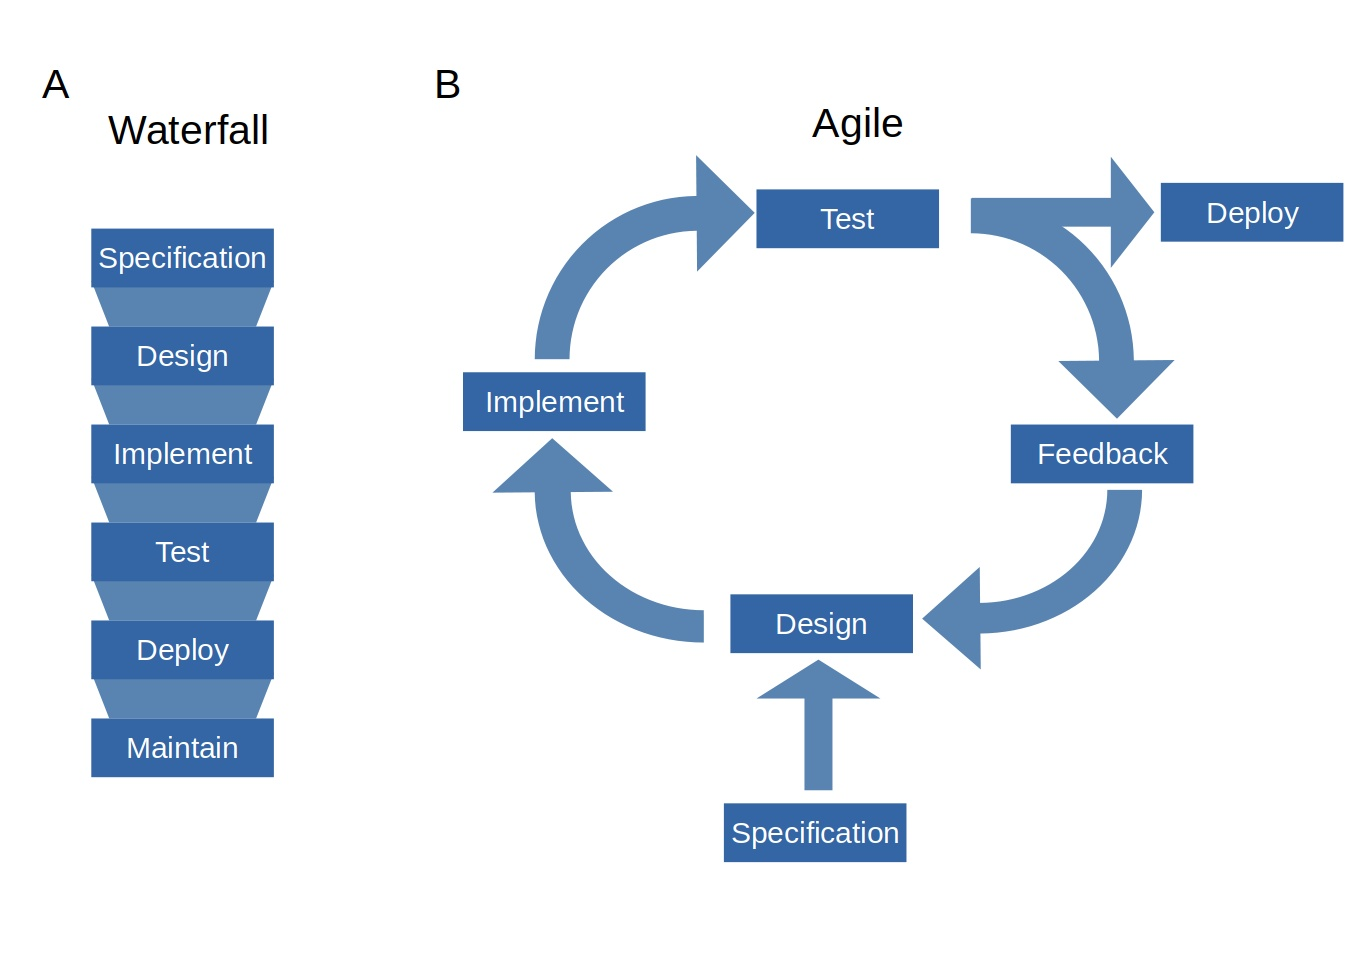
\includegraphics[width=\linewidth]{figures/agileVsWaterfall} 

}

\caption[Summary of Agile and Waterfall software development practices.]{\textbf{Comparison of two common software development practices.} \textbf{A} Waterfall consists of a linear sequence of tasks each of which must be fully completed before moving onto the next. \textbf{B} Agile focuses on gaining feedback as soon as possible by quickly implementing small changes and using feedback to influence the next design stage. }\label{fig:development-practices}
\end{figure}

The simplest software development practice that biologists can implement when writing any code is don't repeat yourself (DRY).
DRY encourages programmers to write short and specific functions to solve regularly occurring tasks. 
Minimising the number of repetitions helps reduce errors; which can be introduced by imperfect copying, improves readability, and enables faster debugging as compartmentalising tasks into separate functions enables you to test each function separately \parencite{Thomas1999}.
However, DRY does have limits as the focus on general abstractions can lead to unreadable code.
For example, a correctly design suite of test is intended to help diagnose bugs during the development stage.
Abstracting error messages to the shortest, most general form can invalid their usefulness in diagnosing bugs.

Research projects that involve more extensive computational analysis can benefit from incorporating the structure given by software development methods used in industry.
A common software development method is called waterfall or plan-driven development.
Waterfall introduces a structure to the coding practice by outlining a series of stages that are completed linearly, Figure \ref{fig:development-practices}A.
It starts with a detailed specification before moving to development and implementation.
Although the traditional implementations of waterfall encourage a strict sequential structure to the completion of a software development task, modified waterfall methods enable a degree of flexibility as adjacent steps can overlap enabling some aspects of the design to change as the software is implemented \parencite{McConnell1996}. 

Agile is an alternative branch of software development methods that focus on getting regular feedback and deviate from the waterfall ethos of leaving testing to a later stage.
They prioritise creating a minimal viable product as soon as possible and testing its functionality.
The specification of an agile project be altered and redefined as the project develops, Figure \ref{fig:development-practices}B. 
The principles behind the agile develop method are outlined in the agile manifesto, \href{https://agilemanifesto.org/principles.html}{agilemanifesto.org}.
Inclusion of agile practices in biomedical research suggests the iterative nature of exploratory research combines effectively with the flexibility of agile software development\parencite{kane2006}.

Two common agile practices in industry that have already been successfully implemented in research software development are scrum and extreme programming \parencite{Sletholt2011,Sadath2018}.
Scrum is the modern archetypal agile method \parencite{Schwaber2020}.
Instead of fixing the development schedule the project is broken into sprints.
Each sprint iteratively adds some functionality which is reviewed, tested and implemented before moving onto the next.
Constantly reviewing and testing the code enables programmers to catch bugs early and to receive feedback on whether the initial functionality is useful and achievable.
As its name suggests extreme programming pushes the principles of agile programming to the extreme \parencite{Beck2004}.
Updates to the software are tested and implemented on a weekly basis. 
In addition, programmers are expected to conduct paired programming; 
two programmers work together at all times with only one coding while the other verbally dictates what should be added. 
Although this reduces the number of lines of code written per developer, constantly reviewing each others code reduces the number of error which is assumed to negate any reduction in productivity.

Despite there being multiple software development methods available in industry, there remains a need for a general method that meets the demands of research software development in an academic environment, \parencite{Cereci2018}. 
The variety of team sizes, project times scales, software development expertise and the usage of research software for exploratory analysis leads to difficulties in finding similarities between projects that can be used to build development methods \parencite{Hannay2009, Diaz2019}.
Hybrid software development methods that combine the overarching structure of waterfall with the flexibility of agile could meet the hypothesis driven and exploratory demands of research software development \parencite{Pathak2012}.

\subsection{Open source software development}

The growing demand for research to be open access has led to almost 25\% of all publication on the web to be openly available in some form \parencite{Khabsa2014}.
The demand for research software that is openly available on public repositories, therefore, is also increasing. 
Open source research software can also have improved findability, accessibility and reproducibility.
Open science research overall is linked with increased citations, funding bodies placing more weight on open access policies and open project tend to get more coverage in the media \parencite{McKiernan2016}.
However, these advantages are only achievable if quality coding practices are implemented using public repositories \parencite{Prlic2012}.
A modern parable for open source software development comes for the epidemiological modelling of the spread of COVID-19 by Prof Neil Ferguson at Imperial Collage London.
Crucial to the justification of national lockdowns to kerb the spread of COVID-19, the model was actual developed 13 years prior using undocumented, closed source C++ code.
After six weeks of intense revisions and refactoring, with direct help from Microsoft and GitHub software architects, the model code is now the perfect example of open source research software \href{https://github.com/mrc-ide/covid-sim}{github.com/mrc-ide/covid-sim}.

\subsection{Software documentation}

\subsubsection{The importance of quality documentation}

The literature on developing useful and usable bioinformatics software is unanimous on the need to document how and why to use a package \parencite{Wilson2017,Taschuk2017,Leprevost2014}.
Furthermore, the widely popular Findable, Accessible, Interoperable and Reusable (FAIR) principles for scientific data now has a similar set for principles for FAIR research software and documentation is at the forefront: "R1. Software is described with a plurality of accurate and relevant attributes" \parencite{Barker2022}.
Widely used software repositories, such as Bioconductor, demand long-form documentation outlining the decisions made in creating a package as well as how to interact with it in order for the package to be accepted \parencite{Gentleman2004}.
Documentation acts as "a resource for learning and a second role: as an advertisement for the software project" and the current health of a project \parencite{Geiger2018}.
As well as being best practice for ensuring code usability, quality documentation can also improve the quality of the code itself.
Documentation of technicalities and a suitable code of conduct can help develop a community of maintainers that can fix bugs, update dependencies and add functionality together \parencite{Community2022}.
Open source documentation also combats unconscious knowledge as developers of the code can overlook key pieces of information for using the software that can only be rectified by new users contributing to the package \parencite{Hermann2022}.


\subsubsection{Factors contributing to poor documentation}

Software is published with inadequate documentation because writing software documentation is a neglected step in software development.
In a 2017 GitHub survey of OSS contributors, 93\% reported that “incomplete or outdated documentation is a pervasive problem” but “60\% of contributors say they rarely or never contribute to documentation” \parencite{Geiger2017}.
Software documentation typically is the least credited part of software development with little time or funds allocated to its development.
In industry, documentation writers are first to go in times of economic difficulty \parencite{Forward2002}.
In academia, research posts are only for a few years so there is little time, or motivation, for the developer to respond to user queries \parencite{Hermann2022}.
Simultaneously, writing software documentation requires the most diverse set of skills and experiences to enable people from different backgrounds and knowledge to engage at an appropriate level \parencite{Geiger2018}.

Software documentation needs to meet multiple demands and engage users with different skill sets in order to be adequate.
Previous research found common issues were based on factually incorrect statements in the documentation, sections of code/functions without any documentation at all or documentation becoming out of date with the latest package versions.
Other issues discuss the difficulty at which API documentation could be found and searched at all, exactly what terms meant in specific contexts and not having quality translations of documentation in other languages.
As expected, a complete lack of documentation is the most common issue but on the other extreme is dense, unintelligible documentation that is difficult to maintain and search \parencite{Aghajani2019}.

\subsection{Suggestions for improving software documentation}

Understanding the purposes of different types of documentation can help improve the overall quality of research software documentation.
Previous studies have recognised three categories of documentation: documentation of decisions, what problem does this software solve and why was this particular method chosen to solve it; documentation of product, what is contained within this software implementation and how do users interact with it; and documentation of technicalities, how did the developers create the software and how can maintainers contribute to it. 
Any software intended to be shared contains some product documentation, but few research software projects outline technical details and fewer still mention any decisions made in development \parencite{Geiger2018}.

Documentation methods need to be developed to structure the writing of documentation to meet the needs of multiple users and tasks.
Diataxis is a framework for creating documentation using its two axes of knowledge: theory vs practice and acquisition vs application. 
They separate software documentation into four rough types: Tutorials, practical, and application knowledge; How-tos, practical, and acquisition knowledge; references, theoretical, and acquisition knowledge; and explanations, theoretical, and application knowledge, \href{https://diataxis.fr/}{diataxis.fr}.
Following a systematic approach to developing software documentation helps projects cover the range of needs of documentation users from first time users to regular maintainers.

The solutions to improving research software documentation target the three main causes: lack of understanding of how to document software, loss of focus on the audience and lack of time time allocated to writing documentation, \parencite{Rios2020}. 
Developers of research software need to be taught the pedagogy of software documentation and the tools available to support documentation.
Institutes such as the Software Sustainability Institute and the Turing Institute are supporting training and learning resources, but little is mentioned in formal data analysis training. 
Similar to the frameworks developed for software development, documentation frameworks need to be popularised to acknowledge the continued effort required to keep documentation relevant, accurate and searchable.

Researchers and software developers need to be rewarded for creating usable and documented software packages.
Recognising and correctly citing the use of software should be as important as citing research papers.
Long-lasting code requires long-term funding which need to be supported by suitable grants judged on appropriate criteria \parencite{Goble2014}.
Funding bodies and journals have acknowledged across the board that research data needs to be FAIR.
The FAIR principles for research software need to be incorporated into funding decisions to reward those who create usable software \parencite{Hong2022}.
Finally, encouraging open source research development will improve documentation as both benefit from contributions from a diversity and inclusive community of maintainers \parencite{Strasser2022}.
\newpage
\end{document}
